\documentclass[10pt, compress]{beamer}

\usepackage{
    algorithm,algorithmic,amsfonts,amsmath,amssymb,bm,booktabs,color,
    enumerate,graphicx,hyperref,microtype,multicol,natbib,nicefrac,url
}
\usepackage[T1]{fontenc}
\usepackage[utf8]{inputenc}

\newcommand{\todo}[1]{\noindent\textbf{\textcolor{red}{(TODO) #1\\}}}

\newcommand{\MDP}{M}
\newcommand{\States}{\mathcal{S}}
\newcommand{\Actions}{\mathcal{A}}
\newcommand{\cost}{C}
\newcommand{\initstatedist}{\rho}
\newcommand{\discount}{\gamma}
\newcommand{\numsamp}{N}
\newcommand{\horizon}{T}
\newcommand{\dynamics}{p}
\newcommand{\policyparams}{\theta}
\newcommand{\policy}{\pi}
\newcommand{\state}{\mathbf{s}}
\renewcommand{\action}{\mathbf{a}}
\newcommand{\costsample}{c}
\newcommand{\policyobj}{\eta}
\newcommand{\dynmodel}{\hat{\dynamics}}
\newcommand{\costmodel}{\hat{\cost}}
\newcommand{\isdmodel}{\hat{\rho}}
\newcommand{\dynmat}{\mathbf{F}}
\newcommand{\dyncovar}{\Sigma}
\newcommand{\costmat}{\mathbf{C}}
\newcommand{\costvec}{\mathbf{c}}
\newcommand{\K}{\mathbf{K}}
\renewcommand{\k}{\mathbf{k}}
\newcommand{\polcovar}{\mathbf{S}}
\newcommand{\latent}{\mathbf{x}}
\newcommand{\traj}{\tau}
\newcommand{\polstepsize}{\epsilon_p}
\newcommand{\modelstepsize}{\epsilon_m}
\newcommand{\R}{\mathbb{R}}
\newcommand{\N}{\mathcal{N}}
\newcommand{\W}{\mathcal{W}}
\renewcommand{\L}{\mathcal{L}}
\newcommand{\E}{\mathbb{E}}
\newcommand{\I}{\mathbb{I}}
\newcommand{\KL}{\text{KL}}
\newcommand{\model}{\mathcal{M}}
\newcommand{\dataset}{\mathcal{D}}
\DeclareMathOperator*{\argmin}{argmin}
\DeclareMathOperator*{\argmax}{argmax}
\newcommand{\colvec}[2][.67]{%
  \scalebox{#1}{%
    \renewcommand{\arraystretch}{.67}%
    $\begin{bmatrix}#2\end{bmatrix}$%
  }
}
\newcommand{\trajectory}{\left[\state_0,\action_0,\ldots,\state_\horizon,\action_\horizon,\state_{\horizon + 1}\right]}
\newcommand{\costtrajectory}{\left[\state_0,\action_0,\costsample_0\ldots,\state_\horizon,\action_\horizon,\costsample_\horizon,\state_{\horizon + 1}\right]}
\newcommand{\latenttrajectory}{\left[\latent_0,\action_0,\ldots,\latent_\horizon,\action_\horizon,\latent_{\horizon + 1}\right]}

\usetheme{metropolis}           % Use metropolis theme

\PassOptionsToPackage{export}{adjustbox}
\usetikzlibrary{fit, positioning}
\usepackage{bm}
\usepackage[mode=buildnew]{standalone}
%\usepackage[export]{adjustbox}
\usepackage{booktabs}
\usepackage[scale=2]{ccicons}
\usefonttheme[onlymath]{serif}
\usepackage{pdfpcnotes}

%\usemintedstyle{trac}

\title{An introduction to the structured variational autoencoder (SVAE)}
\subtitle{}
\date{\today}
\author{Sharad Vikram}
\institute{UCSD}

%\setcounter{tocdepth}{1}

\begin{document}

\begin{frame}
  \titlepage
\end{frame}

\section{Variational inference}

\subsection{Variational message passing}

\begin{frame}{Bayesian inference}
  In Bayesian inference, we compute the posterior
  distribution of observations given data.

  \pause

    \begin{center}
      \includestandalone[width=0.3\textwidth]{tikz/pgm-obs}
    \end{center}
  \pause
  We are interested in the posterior distribution $p(x, y | z)$

  \pause
  This can be computed via Bayes rule:
  \begin{align*}
    p(x, y | z) = \frac{p(x, y, z)}{p(z)} = \frac{p(x)p(y | x)p(z | x, y)}{\int p(x)p(y | x)p(z | x, y)dx dy}
  \end{align*}
\end{frame}

\begin{frame}{Example PGM}
  \textbf{Latent variable model}: Gaussian mixture model
  \begin{columns}
    \begin{column}{0.5\textwidth}
      \begin{center}
        \includestandalone[width=0.6\textwidth]{tikz/gmm}
      \end{center}
    \end{column}
    \begin{column}{0.5\textwidth}
      \begin{align*}
        \pi &\sim \textrm{Dir}(\alpha) \\
        \mu_k, \Sigma_k &\sim \mathcal{NIW}(\psi, \mu_0, \kappa, \nu) \\
        z_i | \pi &\sim \textrm{Cat}(\pi) \\
        x_i | z_i, \bm{\mu}, \bm{\Sigma} \ &\sim \mathcal{N}(\mu_{z_i}, \Sigma_{z_i}) \\
      \end{align*}
    \end{column}
  \end{columns}

  \pause
  \textbf{Local variables}: $\{z_i\}_{i=1}^N$

  \pause
  \textbf{Global variables}: $\pi, \bm{\mu}, \bm{\Sigma}$
\end{frame}

\begin{frame}{Conjugacy}
  \metroset{block=fill}
  \begin{block}{Conjugate}
    Two random variables $x$ and $y$ whose distribution is
    \begin{align*}p(x, y) = p(x)p(y | x)\end{align*} are said to be
      \emph{conjugate} if the posterior $p(x | y)$
    is in the same family of distributions as $p(x)$.
  \end{block}
  \pause
  Examples of conjugate distributions:
  \begin{itemize}
    \item Normal/normal
      \pause
    \item Normal-inverse-wishart(NIW)/normal
      \pause
    \item Dirichlet/multinomial
  \end{itemize}
\end{frame}

\begin{frame}{Exponential family}
  A probability distribution is in the \emph{exponential family}
  if it can be parametrized in the following way.

  \pause

  \begin{align*}
    p(x | \theta) = h(x)\exp\left\{\left\langle\eta(\theta), t_x(x)\right\rangle - \log Z(\eta(\theta))\right\}
  \end{align*}
  where
  \begin{itemize}
      \pause
    \item $h(x)$ - base measure
      \pause
    \item $\eta(\theta)$ - natural parameter function
      \pause
    \item $t_x(x)$ - sufficient statistic function
      \pause
    \item $\log Z(\eta(\theta))$ - log-partition function
  \end{itemize}
  \pause
  \textbf{Examples:} Gaussian, Categorical, Dirichlet, inverse-Wishart
\end{frame}

\begin{frame}{Algorithms for inference}
  Depending on the structure of the graphical model
  and conjugacy of the variables, computing the posterior distribution
  can be easy, or very hard!

  \pause
  Possible ways:
  \begin{itemize}
    \item<2-> Compute posterior analytically
      \pause
    \item<3-> Sampling (MCMC, Gibbs sampling)
      \pause
    \item<4-> Expectation-maximization
      \pause
    \item<5->\alert<6->{Variational inference}
  \end{itemize}
  \pause
\end{frame}

\begin{frame}{Variational inference at a high level}
  For graphical models where we can't compute
  the posterior analytically, \textbf{variational inference}
  is a viable approach.

  \pause
    Consider a latent variable model with global variables
    $\theta$, local variables $z$ and observations $x$. Our desired
    posterior is $p(\theta, z | x)$

    \pause
    \textbf{Strategy}: convert inference into optimization
    \begin{itemize}
        \pause
      \item Instantiate \emph{variational distribution} $q_\phi(\theta, z)$
        where $\phi$ are free parameters
        \pause
      \item Define loss $\textrm{KL}(q_\phi(\theta, z)\|p(\theta, z | x))$
        \pause
      \item Minimize loss $\phi^* = \argmin_\phi \textrm{KL}(q_\phi(\theta, z)\|p(\theta, z | x))$
    \end{itemize}
    \pause
    If $q(\theta, z)$ is sufficiently expressive,
    it can approximate $p(\theta, z | x)$ quite well.
\end{frame}

\begin{frame}{KL-divergence}
  Kullback-Leibler (KL) divergence
  is a measure of how far one probability distribution
  is from another.

  \pause
  For distributions $q(x)$ and $p(x)$,
  \begin{align*}
    \textrm{KL}(q(x)\|p(x)) = \int q(x)\log \frac{q(x)}{p(x)}dx = \E_{q(x)}\left[\log\frac{q(x)}{p(x)}\right]
  \end{align*}

  \pause
  \textbf{Properties:}
  \begin{itemize}
    \item $\textrm{KL}(q(x)\|p(x)) = 0$ if $q(x) = p(x)$.
    \item Asymmetric
  \end{itemize}

\end{frame}

\begin{frame}{Evidence lower bound}
  In general, we cannot even compute $KL(q(\theta, z)\|p(\theta, z | x))$
  because
  we don't know the posterior $p(\theta, z | x)$.

  \pause
  We can rewrite the KL divergence as
  \begin{align*}
    \KL(q(\theta, z)\|p(\theta, z|x)) &= \int q(\theta, z)\log\frac{q(\theta, z)}{p(\theta, z | x)}d\theta, z \\
    %&= \int q(\theta, z) \left(\log q(\theta, z) - \log p(\theta, z | x)\right)d\theta, z \\
    %&= \int q(\theta, z) \left(\log q(\theta, z) - \log \frac{p(\theta, z, x)}{p(x)}\right)d\theta, z \\
    %&= \int q(\theta, z) \left(\log q(\theta, z) - \log p(\theta, z, x) + \log p(x)\right)d\theta, z \\
              &= \log p(x) - \E_{q(\theta, z)}\left[\log\frac{p(x, \theta, z)}{q(\theta, z)}\right]
  \end{align*}

  \pause
  and maximize the \emph{evidence lower bound} (ELBO)
  \begin{align*}
    \L[q(\theta, z)] &= \E_{q(\theta, z)}\left[\log\frac{p(x, \theta, z)}{q(\theta, z)}\right]
  \end{align*}
\end{frame}

\begin{frame}{Picking $q(\theta, x)$}
  How do we pick a $q(\theta, x)$?

  \pause

  In general, a broader $q(\theta, x)$ is harder to optimize.

  \textbf{Options:}
  \begin{itemize}
      \pause
    \item Mean-field ($q(\theta, x) = q(\theta)q(x)$)
      \pause
    \item Conjugate-exponential
      \pause
    \item Differentiable $q$
  \end{itemize}
\end{frame}

\begin{frame}{Mean-field variational inference}
  For a general graphical model
  with variables $\mathbf{X} = \{x_1, x_2, \ldots\}$
  we have joint distribution
  \begin{align*}
    p(\mathbf{X}) = \prod_i p(x_i | \textrm{pa}_i)
  \end{align*}
  where $\textrm{pa}_i$ are the parents of node $x_i$
  in the graph.


  \pause
  Let the set $\mathbf{H}$ be
  all unobserved variables and $\mathbf{V}$ be the observed.


  \pause
  We are interested in the posterior $p(\mathbf{H} | \mathbf{V})$
  and use variational distribution 
  \begin{align*}
    q(\mathbf{H}) = \prod_i q(\mathbf{H}_i)
  \end{align*}


\end{frame}

\begin{frame}{Mean-field variational inference (cont.)}
  The ELBO is now
  \begin{align*}
    \L[q(\mathbf{H})] &= \E_{q(\mathbf{H})} \left[\log\frac{p(\mathbf{H}, \mathbf{V})}{q(\mathbf{H})}\right] \\
                      &= \int\prod_i q(\mathbf{H}_i) \left(\log p(\mathbf{H}, \mathbf{V}) - \log \prod_i q(\mathbf{H}_i)\right)d\mathbf{H}\\
                      &= \int q(\mathbf{H}_j) \left(\int \log p(\mathbf{H}, \mathbf{V})\prod_{i \neq j}q(\mathbf{H}_i)d\mathbf{H}_i \right)d\mathbf{H}_j \\&- \int q(\mathbf{H}_j)\log q(\mathbf{H}_j)d \mathbf{H}_j + \textrm{const.}\\
                      &= \int q(\mathbf{H}_j)\log \tilde{q}(\mathbf{H}_j, \mathbf{V})d \mathbf{H}_j- \int q(\mathbf{H}_j)\log q(\mathbf{H}_j)d \mathbf{H}_j  + \textrm{const.} \\
                      &= -\KL(q(\mathbf{H}_j)\|\tilde{q}(\mathbf{H}_j, \mathbf{V}))  + \textrm{const.}
  \end{align*}
  where 
  \begin{align*}
    \log\tilde{q}(\mathbf{H}_j, \mathbf{V}) = \E_{i \neq j}\left[\log p(\mathbf{H}, \mathbf{V})\right] + \textrm{const.}
  \end{align*}

\end{frame}

\begin{frame}{Optimizing a single factor}
  We can isolate a single factor for each hidden node in the graph $\mathbf{H}_j$.
  This makes optimizing a single variational factor easy!
  \pause
  \begin{align*}
    \L[q(\mathbf{H})] &= -\KL(q(\mathbf{H}_j)\|\tilde{q}(\mathbf{H}_j, \mathbf{V}))  + \textrm{const.}
  \end{align*}
  \pause
  For a single factor $q(\mathbf{H}_j)$, this equation is minimized
  when $q(\mathbf{H}_j) = \tilde{q}(\mathbf{H}_j, \mathbf{V})$.

  \pause
  Furthermore, 
  \begin{align*}
    \log\tilde{q}(\mathbf{H}_j, \mathbf{V}) = \E_{i \neq j}\left[\log p(\mathbf{H}, \mathbf{V})\right] + \textrm{const.}
  \end{align*}
  is a function of only factors other than $q(\mathbf{H}_j)$  and observed data.

  \pause
  \metroset{block=fill}
  \begin{block}{Mean-field variational inference}
    Until converged,
    for each factor $q(\mathbf{H}_j)$,
    hold factors $q(\mathbf{H}_{i \neq j})$ constant and
    set $q(\mathbf{H}_j) = \tilde{q}(\mathbf{H}_j, \mathbf{V})$.
  \end{block}
\end{frame}

\begin{frame}{Conjugate-exponential graphical models}
  If our model is \emph{conjugate-exponential},
  where every node belongs in the exponential
  family of distributions, and is conjugate w.r.t. its parents,
  \begin{align*}
    \log\tilde{q}(\mathbf{H}_j, \mathbf{V}) = \E_{i \neq j}\left[\log p(\mathbf{H}, \mathbf{V})\right] + \textrm{const.}
  \end{align*}

  can be calculated in closed form!
  \pause

  This gives rise to an efficient coordinate-ascent algorithm called variational message passing \cite{vmp} (VMP)
  that can be extended with natural gradients (stochastic variational inference).

\end{frame}

\begin{frame}{Variational message passing}

  An update for node $j$ relies on only its Markov blanket.
  \begin{center}
    \includegraphics<1>[width=0.5\textwidth]{img/vmp-1}
    \includegraphics<2>[width=0.5\textwidth]{img/vmp-2}
    \includegraphics<3>[width=0.5\textwidth]{img/vmp-3}
    \includegraphics<4>[width=0.5\textwidth]{img/vmp-4}
  \end{center}

\end{frame}

\begin{frame}{Messages}
  Let $\eta_j$ is the natural parameter of the distribution $q(\mathbf{H}_j)$.
  \pause
  The message from a parent $Y$ to a child $X$ is
  \begin{align*}
    m_{Y \rightarrow X} = f(\eta_Y)
  \end{align*}
    \pause
  The message from a child $X$ to a parent $Y$ is
  \begin{align*}
    m_{X \rightarrow Y} = g(\eta_X, \{m_{i \rightarrow X}\}_{i \in \textrm{cp}_Y})
  \end{align*}

  \pause
  In conjugate-exponential PGMs, messages can be computed in closed-form.
\end{frame}

\begin{frame}{Summary of VMP}
  \textbf{Setup:} Conjugate-exponential graphical model

  \pause
  \textbf{Problem:} Compute posterior $p(\mathbf{H} | \mathbf{V})$, approximated with $q(\mathbf{H}) = \prod_j q(\mathbf{H}_j)$

  \pause
  \textbf{Solution:} Until converged, for each hidden node $\mathbf{H}_j$:
  \begin{enumerate}
      \pause
    \item Collect messages from children and parents
      \pause
    \item Compute updated distribution parameters from messages
  \end{enumerate}

  \pause
  \textbf{Benefits:} efficient, simple, can incorporate mini-batches (stochastic variational inference)

  \pause
  \textbf{Drawbacks:} can be underexpressive (conjugate-exponential requirement)
\end{frame}

\begin{frame}[standout]
  Demo
\end{frame}

\subsection{Gradient-based variational inference}

\begin{frame}{Monte-Carlo approach}
  The previous approach was \emph{restrictive}! Coordinate ascent only
  works on conjugate-exponential models with the mean-field
  assumption.

  \pause

  Assume a non-conjugate, non-exponential model and a differentiable, sampleable
  $q(\theta, z)$.

  \pause

  \begin{align*}
    \L[q(\theta, z)] &= \E_{q(\theta, z)}\left[\log\frac{p(x, \theta, z)}{q(\theta, z)}\right]
  \end{align*}

  \pause

  Perform Monte-Carlo estimate:
  \begin{align*}
    \hat{\L}[q(\theta, z)] &= \sum_{l = 1}^L {q(\theta^{(l)}, z^{(l)})}\left[\log\frac{p(x, \theta^{(l)}, z^{(l)})}{q(\theta^{(l)}, z^{(l)})}\right]
  \end{align*}
\end{frame}

\begin{frame}{Gradient-based approaches}
  \begin{enumerate}
    \item Start with Monte-Carlo loss
      \begin{align*}
        \hat{\L}[q(\theta, z)] &= \frac{1}{S}\sum_{s = 1}^S {q(\theta^{(s)}, z^{(s)})}\left[\log\frac{p(x, \theta^{(s)}, z^{(s)})}{q(\theta^{(s)}, z^{(s)})}\right]
      \end{align*}
    \item Compute gradient
      \begin{align*}
        \nabla_{\phi}\hat{\L}[q_\phi(\theta, z)] &= \frac{1}{S}\sum_{s = 1}^S \nabla_\phi{q(\theta^{(s)}, z^{(s)})}\left[\log\frac{p(x, \theta^{(s)}, z^{(s)})}{q(\theta^{(s)}, z^{(s)})}\right]
      \end{align*}
    \item Perform gradient ascent
  \end{enumerate}
\end{frame}

\begin{frame}{Issues with gradient-based approaches}
  \textbf{Core problem:}  high-variance gradients

  \pause

  How do we address this?

  \begin{itemize}
    \item Rao-Blackwellization (replace $\E[f(X, Y)]$ with $\E[f(X, Y) | X]$)\cite{blackbox}
    \item Reparametrization trick \cite{vae}
  \end{itemize}
\end{frame}

\begin{frame}{Variational autoencoder}
  The VAE is a generative model for data \cite{vae}.

  \begin{align*}
    z_i &\sim  \N(0, I) \\
    x_i &\sim  \N(\mu_\gamma(z_i), \Sigma_\gamma(z_i))
  \end{align*}
  where $\mu_\gamma$ and $\Sigma_\gamma$ are neural networks parameterized by $\gamma$.

  \pause
  \centering
  \includestandalone[width=0.1\textwidth]{tikz/vae}
  \pause

  How do we do inference?
\end{frame}

\begin{frame}{Variational autoencoder}
  \textbf{Basic strategy:} gradient-based variational inference

  \pause

  \begin{itemize}
    \item Pick $q_\phi(z | x)$ to be a \emph{neural network} parameterized by $\phi$ (both differentiable and sampleable)
  \end{itemize}

  \pause
  Let $r_\phi(x)$ be a neural network (with weights $\phi$)that outputs the parameters to a distribution, for example Gaussian.
  \begin{align*}
    q_\phi(z | x) = \N(r_\phi(x))
  \end{align*}

  \pause

  \begin{itemize}
    \item Use the reparametrization trick to lower variance of gradients
  \end{itemize}
  \pause
  We learn the weights for the two neural networks $(\mu_\gamma(z), \Sigma_\gamma(z))$ and $r_\phi(x)$.
  \pause
  \begin{align*}
    \L[q(z | x)] &= \E_{q(z | x)}\left[\log p(x, z) - \log q(z | x)\right]
  \end{align*}
\end{frame}

\begin{frame}{Reparametrization trick}
  What is the reparametrization trick?
  \pause
  We want to sample $z \sim q(z | x)$ and do so
  it in a roundabout way.
  \begin{align*}
    \epsilon &\sim p(\epsilon) \\
    z &= f(r_\phi(x), \epsilon)
  \end{align*}
  where $\epsilon$ is noise sampled from a simple distribution (e.g. Gaussian)
  and $f$ is a function that depends on the type of distribution.
  \pause
  \metroset{block=fill}
  \begin{block}{Example: sampling from a univariate Gaussian $q_\phi(z | x)$}
    \begin{itemize}
        \pause
      \item Compute $(\mu, \sigma^2) = r(x)$
        \pause
      \item Sample $\epsilon \sim N(0, 1))$
        \pause
      \item Return $z = \mu + \epsilon\sigma$
    \end{itemize}
  \end{block}
  \pause
  This is very effective at decreasing the variance of the gradient.
\end{frame}

\section{Structured variational autoencoder}

\begin{frame}{What is an SVAE?}
  There are two ways of thinking about it
  \begin{itemize}
    \item A conjugate-exponential graphical model
      augmented with a neural network observation model
    \item A VAE augmented with 
      also a graphical
      because of a neural-network observation model
  \end{itemize}

  \pause

  \centering
  \includestandalone[width=0.2\textwidth]{tikz/lgmm}
\end{frame}

\begin{frame}{SVAE GMM}
  \begin{columns}
    \begin{column}{0.5\textwidth}
      \includestandalone[width=0.55\textwidth]{tikz/lgmm}
    \end{column}
    \begin{column}{0.5\textwidth}
      \begin{align*}
        \pi &\sim \textrm{Dir}(\alpha) \\
        \mu_k, \Sigma_k &\sim \mathcal{NIW}(\psi, \mu_0, \kappa, \nu) \\
        z_i | \pi &\sim \textrm{Cat}(\pi) \\
        x_i | z_i, \bm{\mu}, \bm{\Sigma} \ &\sim \mathcal{N}(\mu_{z_i}, \Sigma_{z_i}) \\
        y_i | x_i &\sim \mathcal{N}(\mu_\gamma(x_i), \Sigma(x_i)) \\
      \end{align*}
    \end{column}
  \end{columns}
  \pause
  How do we do inference?
\end{frame}

\begin{frame}{Inference in SVAE}
  Inference in SVAE is a hybrid of gradient-based methods and
  coordinate-ascent.

  \pause

  How do we merge these two different approaches?
  \pause
  \begin{columns}
    \begin{column}{0.25\textwidth}
      \centering
      \includestandalone[width=\textwidth]{tikz/lgmm}
    \end{column}
    \begin{column}{0.75\textwidth}
      \begin{itemize}
          \pause
        \item Learn $q(z_i), q(x_i), q(\pi), q(\mu, \Sigma)$ with stochastic VMP using a neural network 
          $r_\phi(y) = m_{y_i \rightarrow x_i}$
          \pause
        \item Learn weights of neural networks $(\mu_\gamma, \Sigma_\gamma), r_\phi$ using the gradient of the ELBO
      \end{itemize}
    \end{column}
  \end{columns}
\end{frame}

\section{Conclusion}

\subsection{Applications}
\begin{frame}{Why SVAE?}
  The SVAE naturally applies to scenarios where there is already a tractable model.

  \pause
  \begin{center}
    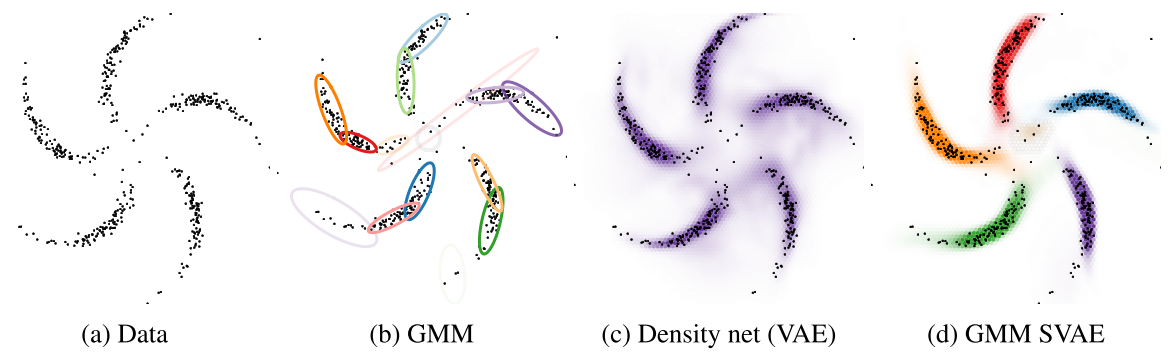
\includegraphics[frame,width=\textwidth]{img/svae-example}
  \end{center}

  \pause
  In this scenario, the SVAE enables modeling non-Gaussian cluster shapes \cite{svae}.
\end{frame}

\subsection{Current work}
\begin{frame}{Current work}
  One idea I am currently working on is using the SVAE to learn
  latent models to be used in reinforcement learning\footnotemark.

  \pause
  \textbf{General approach:}
  \begin{itemize}
    \item Learn a latent LDS
    \item Use MPC to control an agent in the latent space
  \end{itemize}

  \pause
  \textbf{Benefits of this approach:}
  \begin{itemize}
      \pause
    \item We can learn simple dynamics even with camera data
      \pause
    \item Model-based RL tends to be more sample efficient
      \pause
  \end{itemize}
  \pause
  \alert{Demo}
  \footnotetext[1]{Joint work with Marvin Zhang from UC Berkeley}
\end{frame}

\begin{frame}[standout]
  Questions?
\end{frame}

\appendix
\begin{frame}[allowframebreaks]{References}
  \bibliography{main}
  \bibliographystyle{unsrt}
\end{frame}


\end{document}
